\documentclass[12pt]{article}
\usepackage[a4paper, margin=0.75in]{geometry}
\usepackage[document]{ragged2e}
\usepackage{graphicx}
\graphicspath{ {./images/} }
\usepackage{tikz}
\usepackage{caption}
\usetikzlibrary{mindmap}
\usepackage[most]{tcolorbox}
% \usepackage[tmargin=2cm,rmargin=1in,lmargin=1in,margin=0.85in,bmargin=2cm,footskip=.2in]{geometry}
\usepackage{enumerate}
\usepackage{framed}
\usepackage{amsmath,amsfonts,amsthm,thmtools,amssymb,mathtools,commath}
\usepackage{tikz}
\usepackage{xcolor}
\usepackage[most]{tcolorbox}


\tcbuselibrary{theorems}
\newtcbtheorem[number within=section]{example}{Example}%
{
    colback=green!5,
    frame hidden,
    detach title,
    before upper = \tcbtitle\par\smallskip,
    coltitle=green!35!black,
    % colframe=green!35!black,
    fonttitle=\bfseries\sffamily
    % description font=\mdseries
}{th}


\title{
    \textbf{MATH-181} \\
    \textbf{Calculus}
}
\author{
    Note taken by: Turja Roy \\
    ID: 2108052
}
\date{}

\begin{document}
\maketitle

% \tableofcontents

% \newpage
%%%%%%%%%%%
%  Intro  %
%%%%%%%%%%%

\section{Intro}

\begin{minipage}{0.45\textwidth}
    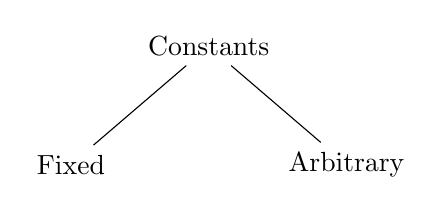
\begin{tikzpicture}
        \node at (0,0){Constants}
        child {node at (-1,0){Fixed}}
        child {node at (1,0){Arbitrary}}
        ;
    \end{tikzpicture}
\end{minipage}
\begin{minipage}{0.45\textwidth}
    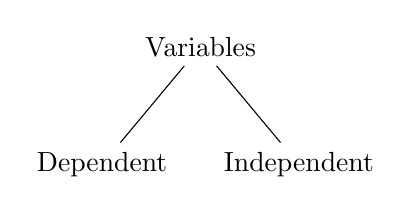
\begin{tikzpicture}
        \node at (0,0){Variables}
        child {node at (2,0){Independent}}
        child {node at (-2,0){Dependent}}
        ;
    \end{tikzpicture}
\end{minipage} \\~\\

\begin{definition*}{Function}

    A rule associating a unique output to a given input.
\end{definition*}


%%%%%%%%%%%%%%%%%%%%%%%%%%%%%%%%%%%%%%%%%%%%%%%%%%
%  Discussion: Examples of Dirichlet and Thomae  %
%%%%%%%%%%%%%%%%%%%%%%%%%%%%%%%%%%%%%%%%%%%%%%%%%%

\subsubsection*{Discussion (A deeper dive): Examples of Dirichlet and Thomae\footnote{Stephen Abbott - Understanding Analysis 4.1}}
Given a function $f$ with domain $A \subseteq \mathbb{R}$, we want to define continuity at a point $c \in A$ to mean that if $x \in A$ is chosen \textit{near c}, then $f(x)$ will be near $f(c)$. \\
Symbolically, we will say $f$ is continuous at $c$ if
$$ \lim_{x \to c} f(x) = f(c) $$
However, the problem is that, at present, it's not entirely clear what is meant by $ \lim_{x \to c} f(x) $. Let's define a function (Idea of German mathematitian Peter Lejuene Dirichlet) $g$ like this:\\
\begin{minipage}{0.45\textwidth}
    \begin{equation*}
        g(x)
        \begin{cases}
            1 & \text{if } x \in \mathbb{Q} \\
            0 & \text{if } x \notin \mathbb{Q}
        \end{cases}
    \end{equation*}
\end{minipage}
\begin{minipage}{0.45\textwidth}
    \centering
    \includegraphics[scale=0.4]{Dirichlet g_x.png}
    \captionof{figure}{\small Dirichlet's Function, $g(x)$}
\end{minipage} \\~\\
Does it make sense to attach a value to the expression $\lim_{x \to 1/2} \ g(x)$? One idea is to consider a sequence $(x_n) \to 1/2$. Using our notion of limit of a sequence if we try to define $g(x_n)$  as simply the limit of the sequence $g(x_n)$, the limit depends on how the sequence $(x_n)$ is chosen. If each $x_n$ is rational, then \[
    \lim_{n \to \infty} g(x_n) = 1
\]
And if $x_n$ is irrational for each n, then \[
    \lim_{n \to \infty} g(x_n) = 0
\]
Generally speaking, we want the value of $\lim_{x \to c} g(x)$ to be independent of how we approach c. In this particular case, the definition of a functional limit that we agree on should lead to the conclusion that \[
    \lim_{x \to 1/2} g(x) \quad\text{does not exist}
\]
We can also realize that Dirichlet's function is not continuous at c = 1/2. In fact, the real significance of the function is that there's nothing unique about the point c=1/2. Because both $\mathbb{Q}$ and $\mathbb{Q}'$ are dense in the real line, it follows that for any $z \in \mathbb{R}$ we can find sequences $(x_n) \subseteq \mathbb{Q}$ and $(y_n) \subseteq \mathbb{Q}'$ such that \[
    \lim x_n = \lim y_n = z
\]
Because \[
    \lim g(x_n) \neq \lim g(y_n)
\]
the same line of reasoning reveals that $g(x)$ is not continuous at $z$. In fact, Dirichlet's function is a \textit{nowhere-continuous} on $\mathbb{R}$.
How about if we redefine the Dirichlet's function in the following way? \\
\begin{minipage}{0.45\textwidth}
    \begin{equation*}
        h(x) = 
        \begin{cases}
            x & \text{ if } x \in \mathbb{Q} \\
            0 & \text{ if } x \notin \mathbb{Q}
        \end{cases}
    \end{equation*}
\end{minipage}
\begin{minipage}{0.45\textwidth}
    \centering
    \includegraphics[scale=0.4]{Dirichlet h_x.png}
    \captionof{figure}{\small Modified Dirichlet's Function, $h(x)$}
\end{minipage} \\~\\
$h$ is not continuous at every point $c \neq 0$ in the same way. \\
But, when $c=0$, these two limits are both equal to $h(0)=0$. Regardless of how we construct a sequence $(z_n)$ converging to zero, the limit is always $\lim h(z_n)=0$. \\
This observation goes to the heart of what we want functional limits to entail. To assert that \[
    \lim_{x \to c} h(x) = L
\]
should imply that \[
    h(z_n) \to L \text{ for all sequences } (z_n) \to c
\]

\quad To this point, we've been discussing continuity of a function at a particular point in its doman. This is a significant departure from thinking of continuous founctions as curves that can be drawn without lifting the pen from the paper, and it leads to some fascinating questions. In 1875, K. J. Thomae discovered the function
\begin{equation*}
    t(x) = 
    \begin{cases}
        1 & \text{ if } x = 0 \\
        1/n & \text{ if } x = m/n \in \mathbb{Q}\backslash \{0\} \text{ is in lowest terms with n $>$ 0 } \\
        0 & \text{ if } x \notin \mathbb{Q}
    \end{cases}
\end{equation*}
\begin{figure}[ht]
    \centering
    \includegraphics[scale=0.5]{Thomae.png}
    \captionof{figure}{\small Thomae's Function, $t(x)$}
\end{figure} \\
If $c \in \mathbb{Q}$, then $t(c) > 0$. Because $\mathbb{Q}'$ is dense in $\mathbb{R}$, we can find a sequence $(y_n)$ in $\mathbb{Q}'$ converging to c. The result is that \[
    \lim t(y_n) = 0 \neq t(c)
\]
and Thomae's function fails to be continuous at any rational point.\\
Let's try this argument on some irrational point like $c=\sqrt{2}$. All irrational values get mapped to $0$ by function $t$, so let's consider a sequence $(x_n)$ of rational numbers instead that converges to $\sqrt{2}$. So, the sequence of rational approximations for $\sqrt{2}$ might be \[
    \left( 1, \frac{14}{10}, \frac{141}{100}, \frac{1414}{1000}, \frac{14142}{10000}, \frac{141421}{100000}, ... \right)
\]
In this case, the sequence $t(x_n)$ begins, \[
    \left( 1, \frac{1}{5}, \frac{1}{100}, \frac{1}{500}, \frac{1}{5000}, \frac{1}{100000}, ... \right)
\]
The denominator of these fractions are getting larger and fast approaching $0 = t(\sqrt{2})$. This always happens. The closer a rational number is chosen to a fixed irrational number, the larger its denominator must necessarily be. Consequently, Thomae's function has the bizarre property of being continuous at every irrational point and discontinuous at every rational point on $\mathbb{R}$. \\

\quad Can there be examples of functions with the opposite property? If we're given some set $A \subseteq \mathbb{R}$, is it always possible to find a function that is continuous only on the set $A^c$? In each of our examples, the functions were defined to have erratic oscillations around points in the domain. What about we restrict our attention to somewhat less volatile functions like a \textit{monotinic} (A function which is either always increasing or always decreasing on a given domain) function? What might we be able to say about the set of discontinuities of a monotonic function on $\mathbb{R}$? \\~\\


%%%%%%%%%%%
%  Limit  %
%%%%%%%%%%%

\section{Limit}

\begin{center}
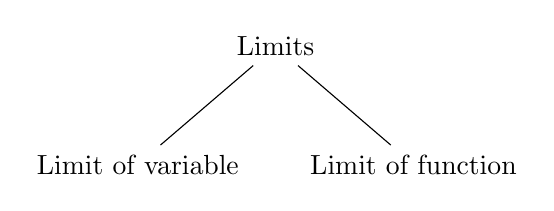
\begin{tikzpicture}
    \node at (0,0){Limits}
    child {node at (-1,0){Limit of variable}}
    child {node at (1,0){Limit of function}}
    ;
\end{tikzpicture}
\end{center}

\begin{definition*}{Limit of variable}

    A constant $a$ is said to be the limit of the variable $x$, if \[
        0 < |x-a| < \delta
    \] where $\delta$ is a pre-assigned positive quantity as small as we please.
\end{definition*}


%%%%%%%%%%%%%%%%%%%%%%%%%
%  Limit of a Sequence  %
%%%%%%%%%%%%%%%%%%%%%%%%%

\subsection{Limit of a Sequence}

\begin{definition}{Sequence}

    A \textit{sequence} is a function whose domain is $N$.\\
    Given a function $f:N \to \mathbb{R}$, $f(n)$ is the $n$th term on the list. The notation for sequences reinforces this familiar Understanding.
\end{definition}

\begin{example}{Each of the following are common ways to describe a sequence}.

    \begin{enumerate}[(i)]
        \item $ \left( 1,\frac{1}{2},\frac{1}{3},\frac{1}{4},\cdots \right)  $
        \item $ \left( \frac{1+n}{n} \right)_{n=1}^{\infty} = \left( \frac{2}{1},\frac{3}{2},\frac{4}{3},\cdots \right)  $
       \item $(a_n)$, where  $a_n=2^n$ for each $n\in \mathbb{N}$
       \item $(x_n)$, where $x_1=2$ and $x_{n+1}=\frac{x_n+1}{2}$
    \end{enumerate}
\end{example}

\begin{definition}{Convergence of a Sequence}
    
    A sequence $(a_n)$ \textit{converges} to a real number $a$ if \[
        \forall\epsilon,\exists N\in\mathbb{N} : n \ge N \implies |a_n-a|<\epsilon
    \] To indicate that $(a_n)$ converges to $a$, we write either $\lim a_n=a $ or $(a_n) \to a$.
\end{definition}

\begin{definition}{$\epsilon$-neighbourhood and $\delta$-neighbourhood}
    
\textbf{$\epsilon$-neighbourhood:}
    \[ \forall \epsilon > 0, U_\epsilon (a) = \{ x\in\mathbb{R} : |x-a| < \epsilon \} = (a-\epsilon, a+\epsilon) \]
    \textbf{$\delta$-neighbourhood:}
    \[ U_\delta(a) = \{x \in \mathbb{R} : |x-a| < \delta \} = (a-\delta, a+\delta) \]

\end{definition}

\begin{definition}{Convergence of a Sequence: Topological Version}
    
    A sequence $(a_n)$ converges to $a$ if, given any $\epsilon$-neighbourhood $U_\epsilon(a)$ of $a$, there exists a point in the sequence after which all of the terms are in $U_\epsilon(a)$. In other words, every $\epsilon$-neighbourhood contains all but a finite number of the terms $(a_n)$.
\end{definition}
\begin{center}
    \includegraphics[scale=0.6]{Limit of a sequence Topological Version.png}
    \captionof{figure}{\small Limit of a sequence}
\end{center} 

The natural number $N$ in the original version of the definition is the point where the sequence $(a_n)$ enters $U_\epsilon(a)$, never to leave. It should be apparent that \textit{the value of $N$ depends on the choice of $\epsilon$}. The smaller the $\epsilon$-neighbourhood, the larger the $N$ may have to be.


%%%%%%%%%%%%%%%%%%%%%%
%  Functional Limit  %
%%%%%%%%%%%%%%%%%%%%%%

\subsection{Functional Limit}
Considering a function $f:A \to R$, a limit point $c$ of $A$ is a point with the property that every $\epsilon$-neighbourhood $U_\epsilon(c)$ intersects $A$ in some point other than $c$. Equivalently, $c$ is a limit point of $A$  if and only if $c=\lim x_n$ for some sequence $(x_n) \subseteq A$ with $x_n \neq c$. \\
\begin{figure}[htpb]
    \centering
    \includegraphics[scale=0.5]{Functional Limit Definition.png}
    \caption{\small Definition of Functional Limit}
\end{figure}

\begin{definition}{$\epsilon-\delta$ Version}

Let $f: A \to \mathbb{R}$ and let c be a limit point of the domain $A$. \[
    \lim_{x \to c} f(x) = L \iff (\forall \epsilon>0, \exists\delta>0 : \forall x \in A, 0 < |x-c| < \delta \implies |f(x)-L| < \epsilon)
\]
Here, \[
    |f(x)-L|<\epsilon \text{ is equivalent to } f(x) \in U_\epsilon(L)
\]
Likewise, \[
    |x-c|<\delta \iff x \in U_\delta(x)
\]
\end{definition}

\begin{definition}{Topological Version}

    Let $f : A \to \mathbb{R}$ and let c be a limit point of the domain of A. We can say, \[
        \lim_{x \to c} f(x)=L \iff ( \forall U_\epsilon(L), \exists U_\delta(c) : \forall x \in A, x \in U_\delta(c) \land x \neq c \implies f(x) \in U_\epsilon(L) )
    \] \\
\end{definition}


\begin{example}{(i) If $f(x) = 3x+1$, prove that $ \lim_{x \to 2} f(x) = 7 $ \\
    (ii) Show that $\lim_{x \to 2} g(x) = 4$ where $g(x)=x^2$.}

    \textbf{(i)} Let $\epsilon>0$. The definition requires we produce a $\delta>0$ so that $0<|x-2|<\delta$ leads to the conclusion $|f(x)-7|<\epsilon$ \[
        |f(x)-7| = |(3x+1)-7| = |3x-6| = 3|x-2|
    \]
    Thus, if we choose $\delta=\epsilon/3$, then $0<|x-2|<\delta$ implies $|f(x)-7|<3(\epsilon/3)=\epsilon$ \\~\\
    
    \textbf{(ii)} Given an arbitrary $\epsilon>0$, our goal is to prove $|g(x)-4|<\epsilon$ by restricting $| x-2 |$ to be smaller than some carefully chosen $\delta$. \[
        |g(x)-4| = |x^2-4| = |x+2||x-2|
    \] We can make $|x-2|$ as small as we like, but we need an upper bound on $|x+2|$ in order to know how small to choose $\delta$. If we agree that our $\delta$-neighbourhood around $c=2$ must have radius no bigger than $\delta=1$, then we get the upper bound $|x+2|\le |3+2|=5$ for all $x\in U_\delta(c)$. \\
    Now, for $\delta=\text{min}(1,\epsilon/5)$, if $0<|x-2|<\delta$, then \[
        |x^2-4| = |x+2||x-2| < (5)\frac{\epsilon}{5} = \epsilon
    \] and hence, the limit is proved. \\~\\
\end{example}

\begin{example}{From the definition of $(\delta,\epsilon)$ show that $\lim_{x \to 3} (2x^3-3x^2-18x+29)=2$}

    Let for a given $\epsilon>0$, however small $0<|x-3|<\lambda<1$ ------(1)
    \begin{align*}
        \therefore |2x^3-3x^2-18x+29 - 2| &= |2x^3-3x^2-18x+27| \\
        &= |2(x-3)^3 + 15(x-3)^2 + 18(x-3)| \\
        &\le 2(x-3)^3 + 15(x-3)^2 + 18(x-3) \\
        &\le 2\lambda^3 + 15\lambda^2 + 18\lambda \\
        &< 35\lambda \quad\quad\quad [ \because \lambda^3<\lambda^2<\lambda<1 ]
    \end{align*}
    Now, $|2x^3-3x^2-18x+29|<\epsilon$, where $\epsilon=35\lambda$ ------(2) \\
    or, $\lambda=\epsilon/35$. Therefore, we can determine a small positive number $\delta$ depending on $\epsilon$ such that the limit is established. Here $\delta=\epsilon/35$. Hence it's proved that \[
        \lim_{x \to 3} (2x^3-3x^2-18x+29) = 2 \quad\quad \text{[From (1) and (2)]}
    \]
\end{example}


%%%%%%%%%%%%%%%%%%%%%%%%%%%%%%%%%%%%%%%%%%
%  Left Hand Limit and Right Hand Limit  %
%%%%%%%%%%%%%%%%%%%%%%%%%%%%%%%%%%%%%%%%%%

\subsubsection{Left hand limit and Right hand limit}

Informally speaking, we can say $L^-$ is the LHL of the function $f$ at a point $a$ if we can get $f(x)$ as close as we want to $L$ by taking $a$ to the left of $x$ and close to $x$, but not equal to $a$, and we write \[
    \lim_{x \to a^-} f(x) = L^-
    \] In the same way, we can say $L^+$ is the RHL of the function if we take a to the right, and we write \[
    \lim_{x \to a^+} f(x) = L^+
\]

\begin{definition}{Left Hand Limit}

    \[ L^- = \lim_{x \to a^-} f(x) \iff \left( \forall\epsilon>0,\exists\delta : \forall x, 0<(a-x)<\delta \implies |f(x)-L^-|<\epsilon \right) \]
\end{definition}
\begin{definition}{Right Hand Limit}

\[
    L^+ = \lim_{x \to a^+} f(x) \iff \left( \forall\epsilon>0,\exists\delta : \forall x, 0<(x-a)<\delta \implies |f(x)-L^+|<\epsilon \right) 
\]
\end{definition}

\begin{figure}[htpb]
    \centering
    \includegraphics[scale=0.5]{Limit1.png}
    \caption{\small Left and Right Hand Limit}
\end{figure}
\[ |x-5| < \epsilon \]
\[ -\epsilon < x-5 < \epsilon \]
\[ 5-\epsilon < x < 5+\epsilon \]

\begin{theorem}{Relation between one-sided and two-sided limits}
    
    Limit of a function at point $a$ exists if:
    \begin{enumerate}[(i)]
        \item $\lim_{x \to a^-} f(x)$ exists
        \item $\lim_{x \to a^+} f(x)$ exists
        \item $\lim_{x \to a^-} = \lim_{x \to a^+}$ 
    \end{enumerate}
    That is, \[
        \lim_{x \to a} f(x) = L \iff \lim_{x \to a^-} f(x) = \lim_{x \to a^+} f(x) = L 
    \]
\end{theorem} \\~\\

\begin{minipage}{0.6\textwidth}
    \begin{alignat*}{2}
             & \text{\underline{Put x=1}}\\
             & \frac{x^2-1}{x-1} &&\to \frac{0}{0} \to \text{Apply L'H\^ospital} \\
        x\to1 \quad & \frac{x^2-1}{x+1} &&\to \frac{0}{2} \to \text{Limit exists} \\
             & \frac{x^2+1}{x^2-1} &&\to \frac{2}{0} \to \text{Limit doesn't exist} \\
    \end{alignat*}
\end{minipage}
\begin{minipage}{0.3\textwidth}
    \textbf{Use L'H\^opital Rule}\\
    \underline{The 7 Indeterminate forms} \\
    \begin{enumerate}[(1)]
        \item $\frac{0}{0}$ 
        \item $\frac{\infty}{\infty}$ 
        \item $0 \times \infty$ 
        \item $\infty-\infty$
        \item $1^{\infty}$ 
        \item $0^0$ 
        \item $\infty^0$
    \end{enumerate}
\end{minipage}

\begin{example}{
        Investigate the following function at $x=0$ and $x=\frac{1}{2}$ \\
        \begin{equation*}
            f(x)
            \begin{cases}
                1+2x, &\text{ for }-\frac{1}{2}\le x<0 \\
                1-2x, &\text{ for }0\le x<\frac{1}{2} \\
                -1+2x &\text{ for }x>\frac{1}{2}
            \end{cases}
        \end{equation*}
    }

        For $x=0$ :
        \[ \text{LHL} = \lim_{x \to 0^-} f(x) = \lim_{x \to 0^-} \{ 1 + 2 \times 0 \} = 1 \]
        \[ \text{RHL} = \lim_{x \to 0^+} f(x) = \lim_{x \to 0^+} \{ 1 - 2 \times 0 \} = 1 \]
        \[ f(0) = 1-2\times0 = 1 \]
        Thus we get, $\lim_{x \to 0} f(x) = 1 = f(0)$. i.e The function is continuous at $x=0$ \\~\\

        For $x=\frac{1}{2}$ :
        \[ \text{LHL} = \lim_{x \to \frac{1}{2}^-} f(x) = \lim_{x \to \frac{1}{2}^-} \left\{ 1 - 2\left( \frac{1}{2} \right)  \right\} = 0 \]
        \[ \text{RHL} = \lim_{x \to \frac{1}{2}^+} f(x) = \lim_{x \to \frac{1}{2}^+} \left\{ -1 + 2\left( \frac{1}{2} \right)  \right\} = 0 \]
        As LHL=RHL, we can say that limit exists at $x=\frac{1}{2}$. However, the function is discontinuous at $x=\frac{1}{2}$ since $f\left( \frac{1}{2} \right) $ doesn't exist.
\end{example}

\begin{theorem}{Fundamental Theorems on Limits}
    
    If $\lim_{x \to a} f(x) = l$ and $\lim_{x \to a} g(x) = m$, where $l$ and $m$ are finite quantities and $c$ is a constant,
    \begin{enumerate}[(i)]
        \item $ \lim_{x \to a} \{ f(x) \pm g(x) \} = l \pm m $
        \item $ \lim_{x \to a} \{ f(x)g(x) \} = lm $ 
        \item $ \lim_{x \to a} \left\{ \frac{f(x)}{g(x)} \right\} = \frac{l}{m} $, provided $g(x)\neq 0$
        \item $ \lim_{x \to a} c = c $
        \item $ \lim_{x \to a} c f(x) = c \lim_{x \to a} f(x) $
        \item $ \lim_{x \to a} \left( f(x) \right)^n = \left( \lim_{x \to a} f(x) \right)^n $
        \item $ \lim_{x \to a} \sqrt[n]{f(x)} = \sqrt[n]{\lim_{x \to a} f(x)} $, provided $\lim_{x \to a} f(x) > 0$
    \end{enumerate}
\end{theorem}

\begin{theorem}{The Squeeze/Sandwitch Theorem}
   
    If there is a $c>0$ such that \[
        f(x)\le g(x)\le h(x)
    \] for all $x\in(a-c,a)\cup(a,a+c)$ (i.e $x$ in a deleted neighbourhood of $c$), if \[
        \lim_{x \to a} f(x) = \lim_{x \to a} h(x) = L \text{, then } \lim_{x \to a} g(x) = L
    \]
    \begin{center}
        \includegraphics[scale=0.5]{SqueezeTheorem.png}
        \captionof{figure}{\small Squeeze Theorem}
    \end{center}
\end{theorem} \\~\\


%%%%%%%%%%%%%%%%
%  Asymptotes  %
%%%%%%%%%%%%%%%%

\subsubsection{Asymptotes}
Greek \textit{asymptotos} means `nonintersecting'. Asymptote is infinitesimally close to a curve, but never touches it.

\begin{definition}{Asymptote}

    An asymptote of a curve $f(x)$ is a line such that the distance between the curve and the line approaches zero as one or both of the $x$ and $y$ coordinates approach infinity. \\
    There are 3 types of asymptotes:
    \begin{enumerate}
        \item Vertical asymptote
        \item Horizontal asymptote
        \item Oblique asymptote
    \end{enumerate}
\end{definition}

\begin{center}
    \includegraphics[scale=0.4]{Types of asymptotes.png}
    \captionof{figure}{\small Types of asymptotes}
\end{center}

\begin{definition}{Vertical asymptote}
    
    The line $x=a$ is a vertical asymptote of the function $f(x)$ if $f$ approaches infinity as $x$ approaches $a$. That is, either \[
        \lim_{x \to a^-} f(x) = \pm \infty, \text{ or } \lim_{x \to a^+} f(x) = \pm \infty, \text{ or both. }
    \]
\end{definition}
\begin{definition}{Horizontal asymptote}

    The horizontal line $y=c$ is a horizontal asymptote of the function $g(x)$ if \[
        \lim_{x \to -\infty} g(x) = c, \text{ or } \lim_{x \to +\infty} g(x) = c
    \]
\end{definition}
\begin{definition}{Oblique asymptote}

    A function $f(x)$ is asymptotic to the straight line $y=mx+b$ $(m \neq 0)$ if \[
        \lim_{x \to +\infty} [ f(x) - (mx+b) ] = 0, \text{ or } \lim_{x \to -\infty} [ f(x) - (mx+b) ] = 0
    \]
\end{definition}

\begin{minipage}{0.32\textwidth}
    \begin{center}
        \includegraphics[scale=0.2]{Vertical asymptotes.jpg}
        \captionof{figure}{\small Vertical asymptote}
    \end{center}
\end{minipage}
\begin{minipage}{0.33\textwidth}
    \begin{center}
        \includegraphics[scale=0.2]{Horizontal asymptotes.jpg}
        \captionof{figure}{\small Horizontal asymptote}
    \end{center}
\end{minipage}
\begin{minipage}{0.33\textwidth}
    \begin{center}
        \includegraphics[scale=0.3]{Oblique asymptotes.jpeg}
        \captionof{figure}{\small Oblique asymptote}
    \end{center}
\end{minipage}

%%%%%%%%%%%%%%%%%%%%%%%%
%  End Behavior Model  %
%%%%%%%%%%%%%%%%%%%%%%%%

\subsubsection{End Behavior Model}
For numerically large values of $x$, we can sometimes model the behavior of a complicated function by a simpler one that acts virtually in the same way.

\begin{example}{Let $f(x) = 3x^4 - 2x^3 + 3x^2 - 5x + 6$ and $g(x) = 3x^4$. Show that while $f$ and $g$ are quite different for numerically small values of $x$, they are virtually identical for $|x|$ large.}
    
    We can test the claim that $g(x)$ models $f(x)$ for numerically large values of $x$ by taking the ratio of the functions as $x \to \pm \infty$. \\
    \begin{align*}
        \lim_{x \to \pm\infty} \frac{f(x)}{g(x)} &= \lim_{x \to \pm\infty} \frac{3x^4-2x^3+3x^2-5x+6}{3x^4} \\
        &= \lim_{x \to \pm\infty} \left( 1 - \frac{2}{3x} + \frac{1}{x^2} - \frac{5}{3x^3} + \frac{2}{x^4} \right)  \\
        &= 1 \\
    \end{align*}
    convincing evidence that $f$ and $g$ behave alike for $|x|$ large.
\end{example}

\begin{definition}{End Behavior Model}

    The function $g(x)$ is a
    \begin{enumerate}[(a)]
        \item left end behavior model for f(x) if and only if \[ \lim_{x \to -\infty} \frac{f(x)}{g(x)} = 1 \]
        \item right end behavior model for f(x) if and only if \[ \lim_{x \to +\infty} \frac{f(x)}{g(x)} = 1 \]
    \end{enumerate}
    If $g(x)$ provides both a left and a right end behavior model, it is simply called an \textbf{End Behavior Model}.
\end{definition}

\begin{example}{Find an end behavior model for
    \begin{enumerate}[(a)]
        \item $f(x) = \frac{2x^5+x^4-x^2+1}{3x^2-5x+7}$
        \item $g(x) = \frac{2x^3-x^2+x-1}{5x^3+x^2+x-5}$
    \end{enumerate}}
    
    \textbf{(a)} $2x^5$ is an end behavior model for the numerator of $f$, and $3x^2$ for the denominator. This makes \[
        \frac{2x^5}{3x^2} = \frac{2}{3}x^2
    \] an end behavior model for $f$. \\~\\
    \textbf{(b)} $2x^3$ is an end behavior model for the numerator of $g$, and $5x^3$ for the denominator. This makes \[
        \frac{2x^3}{5x^3} = \frac{2}{5}
    \] an end behavior model for $g$.
\end{example}

\begin{example}{Let $f(x)=x+e^{-x}$. Show that $g(x)=x$ is a right end behavior model for $f$ while $h(x)=e^{-x}$ is a left end behavior model for $f$.}
    
    On the right, \[
        \lim_{x \to \infty} \frac{f(x)}{g(x)} = \lim_{x \to \infty} \frac{x+e^{-x}}{x} = \lim_{x \to \infty} \left( 1+\frac{e^{-x}}{x} \right) = 1
    \] On the left, \[
        \lim_{x \to -\infty} \frac{f(x)}{h(x)} = \lim_{x \to -\infty} \frac{x+e^{-x}}{e^{-x}} = \lim_{x \to -\infty} \left( \frac{x}{e^{-x}}+1 \right) = 1
    \]
\end{example}


%%%%%%%%%%%%%%%%%%%%%%%%%%%%%%%%%%
%  Continuity and Discontinuity  %
%%%%%%%%%%%%%%%%%%%%%%%%%%%%%%%%%%

\section{Continuity and Discontinuity}

\begin{definition}{Continuity}
    
    \\ A function $f(x)$ is said to be continuous at $x=a$ if,
    \begin{enumerate}[(i)]
        \item $\lim_{x \to a^-} f(x)$ exists
        \item $\lim_{x \to a^+} f(x)$ exists
        \item $f(x)$ is finite
        \item $\lim_{x \to a^-} f(x) = f(a) = \lim_{x \to a^+} f(x)$
    \end{enumerate}
\end{definition}

\begin{theorem}{Classification of Discontinuity}

    \begin{enumerate}[(i)]
        \item Ordinary discontinuity / discontinuity of 1st order
        \item Ordinary discontinuity / discontinuity of 2nd order
        \item Removal discontinuity
        \item Mixed discontinuity
        \item Oscillatory discontinuity
        \item Infinite discontinuity
    \end{enumerate}
\end{theorem}





\end{document}
